\documentclass[a5paper]{article}
\usepackage[a5paper, top=8mm, bottom=8mm, left=8mm, right=8mm]{geometry}

\usepackage{polyglossia}
\setdefaultlanguage[babelshorthands=true]{russian}

\usepackage{fontspec}
\setmainfont{FreeSerif}
\newfontfamily{\russianfonttt}[Scale=0.7]{DejaVuSansMono}

\usepackage[font=scriptsize]{caption}

\usepackage{amsmath}
\usepackage{amssymb,amsfonts,textcomp}
\usepackage{color}
\usepackage{array}
\usepackage{hhline}
\usepackage{cite}
\usepackage{textcomp}

\usepackage[hang,multiple]{footmisc}
\renewcommand{\footnotelayout}{\raggedright}

\PassOptionsToPackage{hyphens}{url}\usepackage[xetex,linktocpage=true,plainpages=false,pdfpagelabels=false]{hyperref}
\hypersetup{colorlinks=true, linkcolor=blue, citecolor=blue, filecolor=blue, urlcolor=blue, pdftitle=1, pdfauthor=, pdfsubject=, pdfkeywords=}

\newlength\Colsep
\setlength\Colsep{10pt}

\usepackage{tabu}

\usepackage{graphicx}
\usepackage{indentfirst}
\usepackage{multirow}
\usepackage{subfig}
\usepackage{footnote}
\usepackage{minted}
\usepackage{xcolor}

\newcommand{\todo}[1] {
\begin{center}\textcolor{red}{TODO: #1}\end{center}
}

\newcommand{\attribution}[1] {
    \vspace{-5mm}\begin{flushright}\begin{scriptsize}\textcolor{gray}
    {\textcopyright\, #1}\end{scriptsize}\end{flushright}
}

\sloppy
\pagestyle{plain}

\title{Лекция 10: Архитектурные стили}
\author{Юрий Литвинов\\\small{yurii.litvinov@gmail.com}}
\date{}

\begin{document}

\maketitle
\thispagestyle{empty}

\section{Архитектурные шаблоны и стили}

Эта лекция --- пожалуй, самая <<архитектурная>> в этом курсе, на ней пойдёт речь о наиболее известных архитектурных стилях. Вообще, архитектурный стиль --- это набор решений, которые:

\begin{enumerate}
    \item применимы в выбранном контексте разработки,
    \item задают ограничения на принимаемые архитектурные решения, специфичные для определённых систем в этом контексте,
    \item приводят к желаемым положительным качествам получаемой системы.
\end{enumerate}

Есть ещё архитектурные шаблоны --- это именованный набор ключевых проектных решений по эффективной организации подсистем, применимых для повторяемых технических задач проектирования в различных контекстах и предметных областях.

Определения довольно размытые, но суть дела поясняет рисунок:

\begin{center}
    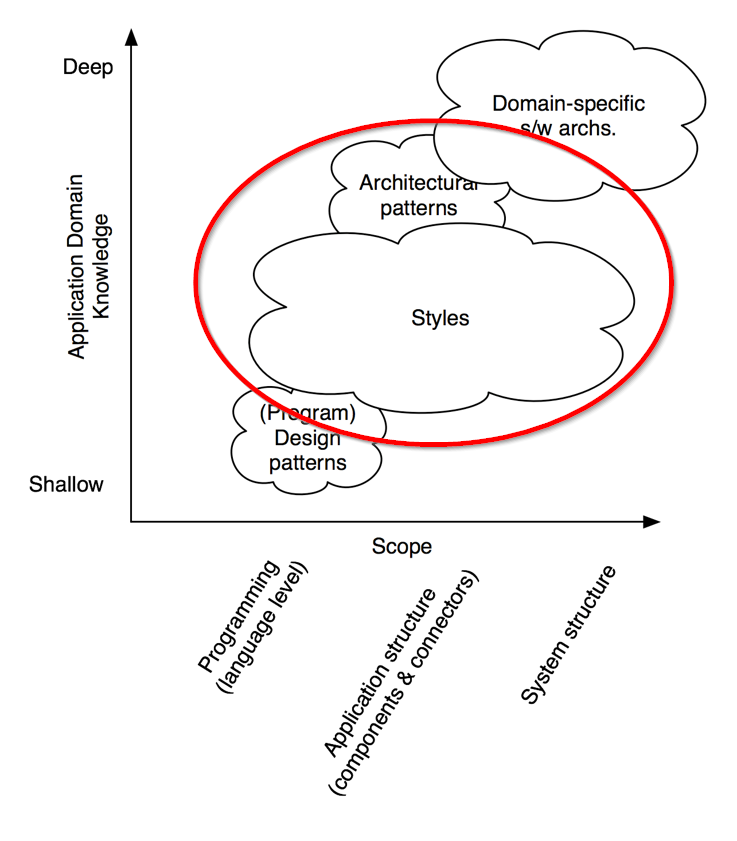
\includegraphics[width=0.7\textwidth]{architecturalStylesHighlighted.png}
    \attribution{N. Medvidovic}
\end{center}

Паттерны проектирования, которые мобсуждались в предыдущих лекциях --- самые <<тактические>> элементы архитектуры. Они никак не привязаны к предметной области и появляются на уровне реализации небольших подсистем или даже конкретных классов. Архитектурные стили, о которых в основном пойдёт речь сегодня, применимы уже не для всех проектов вообще, а в предпочтительных для каждого стиля предметных областях --- одни стили хорошо работают во встроенных системах, другие --- сетевых приложениях, третьи --- в информационных системах (отсюда <<применимы в выбранном контексте разработки>> из определения). И решения, диктуемые стилями, применяются не на уровне конкретных классов, а на уровне подсистем или даже целой системы.

Архитектурные шаблоны --- это более специализированная вещь, чем стили, и несколько более <<тактическая>> (хотя и не настолько, как паттерны). Архитектурные шаблоны диктуют типовые решения для типовых задач, например, организация системы в виде тройки Sense-Ccompute-Control в робототехнике, или Model-View-Controller в пользовательских интерфейсах. Model-View-Controller не претендует на то, чтобы диктовать архитектуру всего приложения, и тем отличается от архитектурных стилей --- обычно MVC лишь вершина айсберга, ответственная за общение с пользователем, а настоящая Архитектура начинается на уровне бизнес-логики, с которым работает Model.

Ещё выше по масштабности и глубже по погружению в предметную область находятся предметно-ориентированные архитектуры или Reference Architectures (например, Space AVionics Open Interface aRchitecture от ESA, Connected Vehicle Reference Implementation Architecture и т.д. и т.п.). В каждой предметной области они свои и, как правило, даже диктуются стандартами. Рассматривать их в этом курсе мы не будем в силу их чрезмерной специфичности.

\section{Архитектурные шаблоны}

Вот несколько примеров архитектурных шаблонов. Они тоже специфичны для предметных областей, но некоторые часто встречающиеся достойны рассмотрения.

\subsection{State-Logic-Display}

\noindent\begin{minipage}{\textwidth}
    \begin{minipage}[c][6cm][c]{\dimexpr0.7\textwidth-0.5\Colsep\relax}
        State-Logic-Display, также известный как <<трёхзвенная архитектура>>, часто рассматривается как архитектурный стиль, часто --- как архитектурный шаблон, так что вообще разделение на архитектурные шаблоны и архитектурные стили весьма условно. Многие приложения могут целиком быть реализованы по трёхзвенной схеме, причём ни в одном из этих звеньев не будет содержательной архитектурной сложности, тогда это что-то вроде стиля. Если трёхзвенка --- это только способ решения одной из задач, то это архитектурный шаблон.
    \end{minipage}\hfill
    \begin{minipage}[c][6cm][c]{\dimexpr0.3\textwidth-0.5\Colsep\relax}
        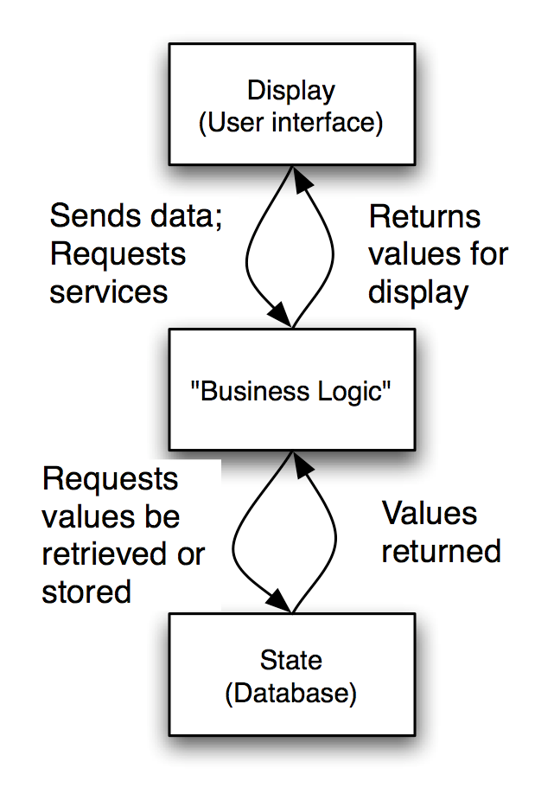
\includegraphics[width=0.9\textwidth]{threeTieredArchitecture.png}
    \end{minipage}%
\end{minipage}

\end{document}
